\chapter{Thực nghiệm}
Với mục tiêu tìm hiểu và giải quyết bài toán phân loại thực khuẩn với dữ liệu đầu vào là contig, nhóm sinh viên thực hiện các thử nghiệm và đánh giá tương tự với nhóm tác giả DeePhage. Chương này trình bày phương pháp xây dựng bộ dữ liệu, các chỉ số đánh giá, kịch bản và kết quả thực nghiệm.

\section{ Xây dựng bộ dữ liệu}
\subsection{ Xử lý nhãn }
Sau khi tìm hiểu các bài báo, nhóm sinh viên thực hiện xây dựng bộ dữ liệu mới dựa trên 2 bộ dữ liệu được sử dụng trong bài báo DeepPL và DeePhage. Nhãn $y$ của bản ghi $X$ được nhóm sinh viên xử lý như sau:
\begin{enumerate}
    \item Nếu $X \in DeePhage \Rightarrow y = y_{DeePhage}$ 
    \item Nếu $X \in DeepPL \Rightarrow y = y_{DeepPL}$
    \item Nếu $X \in DeePhage \cap DeepPL \Rightarrow y = y_{DeePhage}$
\end{enumerate}

\subsection{ Chia tập dữ liệu}
Sau khi thực hiện gộp 2 bộ dữ liệu DeePhage và DeepPL, nhóm sinh viên xử lý dữ liệu theo 4 bước sau:
\begin{enumerate}
    \item Chia bộ dữ liệu thành 2 tập: huấn luyện và kiểm thử.
    \item Sử dụng kỹ thuật cửa sổ trượt, tạo các đoạn contig từ bộ gen đầy đủ với 4 nhóm độ dài khác nhau. Khi thực hiện tạo ra các contig, nhóm đã cài đặt đoạn cửa sổ sau sẽ có sự trùng lặp 30\% so với đoạn cửa số trước và phân bố độ dài các contig trong 1 nhóm tuân theo phân bố chuẩn.
    \begin{itemize}
        \item A: 100 bp - 400 bp
        \item B: 400 bp - 800 bp
        \item C: 800 bp - 1200 bp
        \item D: 1200 bp - 1800 bp
    \end{itemize}
    \item Thực hiện véc-tơ hóa dữ liệu. Tại bước này, nhóm sinh viên sử dụng 2 phương pháp véc-tơ hóa dữ liệu: One-hot và Word2Vec để phù hợp với 2 kịch bản thực nghiệm được trình bày tại phần \ref{ kịch bản thực nghiệm}
    \begin{itemize}
        \item Sử dụng One-hot đối với phương pháp DeePhage.
        \item Sử dụng Word2Vec với k-mer=6.
    \end{itemize}
    \item Áp dụng Random Undersampling để cân bằng phân phối nhãn của bộ dữ liệu.
\end{enumerate}

\section{Kịch bản thực nghiệm}\label{ kịch bản thực nghiệm}
Để tiến hành các thực nghiệm, nhóm sinh viên chọn 2 mô hình là DeePhage và XGBoost. Nhận thấy DeePhage là công cụ toàn diện hơn so với nhóm công cụ dựa trên Bert do DeePhage có thể thực hiện phân loại trên nhiều nhóm contig có đội dài linh hoạt, trong khi nhóm công cụ dựa trên Bert chỉ được đánh giá trên bộ dữ liệu có độ dài đầu vào nhỏ hơn bằng 512 bp, nhóm sinh viên quyết định chọn DeePhage là công cụ tiêu chuẩn trong các thực nghiệm. Ngoài ra, do cần 1 mô hình đủ mạnh để có thể có hiệu suất phân loại tốt cũng như nhanh trong quá trình huấn luyện, nhóm quyết định chọn XGBoost là mô hình được sử dụng để trực tiếp so sánh với DeePhage.

Nhóm sinh viên thực hiện 3 kịch bản: 1 - thực hiện kiểm nghiệm lại kết quả công bố của mô hình DeePhage, 2 - so sánh hiệu suất phân loại của DeePhage và XGBoost trên tập dữ liệu xây dựng. Với kịch bản 1, mục tiêu của nhóm sinh viên là xác thực lại kết quả mà nhóm tác giả công bố. Ngoài ra, do mã nguồn mà nhóm tác giả công bố sử dụng thư viện Tensorflow với phiên bản không hỗ trợ phần cứng hiện có, nên nhóm sinh viên cần cài đặt lại mã nguồn dựa trên Pytorch. Vì vậy, việc thực hiện kịch bản 1 là cách để kiểm thử mã nguồn mới. Kịch bản 2 được thực hiện để có cái nhìn so sánh giữa mô hình DeePhage và XGBoost trên tập dữ liệu mà nhóm sinh viên xây dựng. Đối với DeePhage, dữ liệu được tiền xử lý với phương pháp mã hóa One-hot, phương pháp Word2Vec được sử dụng để mã hóa dữ liệu khi thực hiện với XGBoost.

\section{Các chỉ số đánh giá}
Để đánh giá 1 cách toàn diện hiệu suất phân loại của mô hình chứ không chỉ tập trung vào nhãn 1, nhóm sinh viên sử dụng các chỉ số sau:
\begin{itemize}
    \item Accuracy: sử dụng để do lường hiệu suất phân loại chung của mô hình trên 2 nhãn.
    \item Sensitivity: sử dụng để đo lường dộ phủ của mô hình trên nhãn 1.
    \item Specificity: sử dụng để đo lường độ phủ của mô hình trên nhãn 0.
\end{itemize}
Ngoài những chỉ số trên, các chỉ số Precision, F1, ROC\_AUC cũng được sử dụng trong kịch bản 2.

\section{Kết quả}
\subsection{Hiệu suất phân loại của DeePhage trên bộ dữ liệu xây dựng}

\begin{figure}[H]
    \centering
    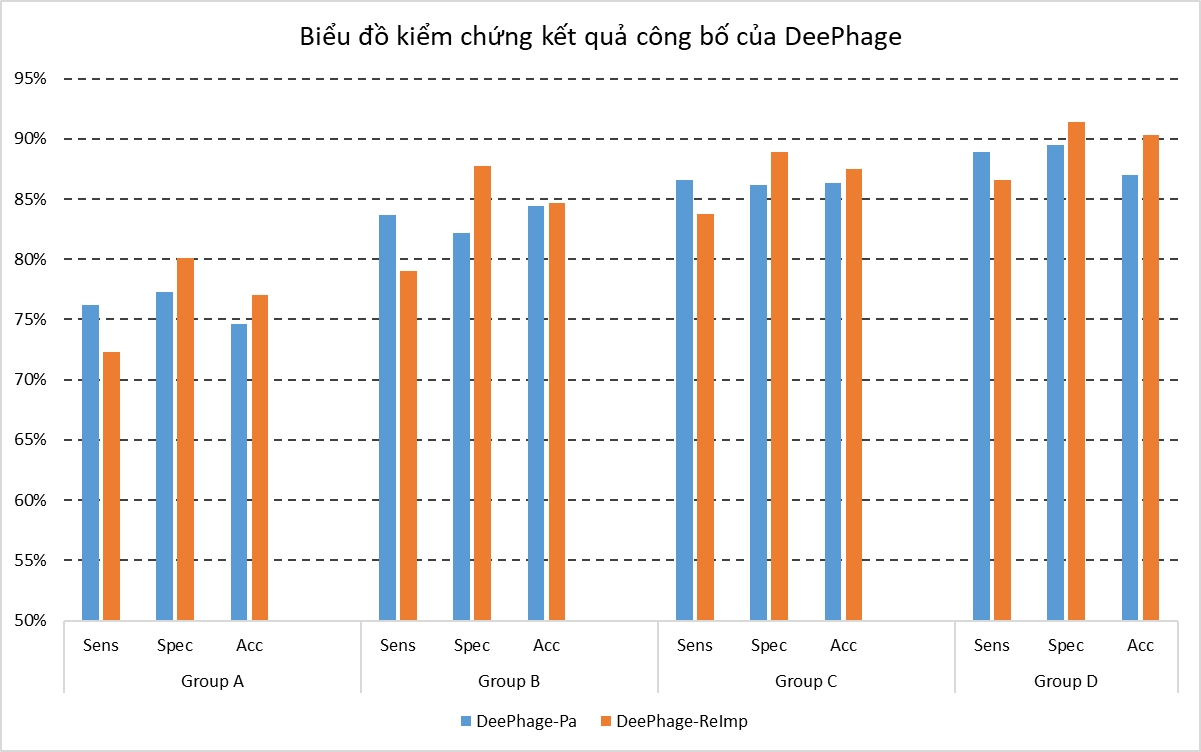
\includegraphics[width=1\linewidth]{figures/result_verify_deephage.png}
    \caption{So sánh hiệu suất phân loại của mô hình DeePhage trên 2 bộ dữ liệu xây dựng và công bố.}
    \label{fig:result_1}
\end{figure}

Hình \ref{fig:result_1} là biểu đồ so sánh kết quả công bố của DeePhage (DeePhage-Pa) và kết quả mô hình được cài đặt lại (DeePhage-ReImp). Kết quả cho thấy mức độ chênh lệch ở mức hợp lý, không quá 5\%. Từ đây có thể kết luận rằng, mã nguồn mà nhóm sinh viên cài đặt lại phù hợp để sử dụng cho các thực nghiệm kế tiếp.

\subsection{So sánh hiệu suất phân loại giữa DeePhage và XGBoost trên bộ dữ liệu xây dựng}

\begin{figure}[H]
    \centering
    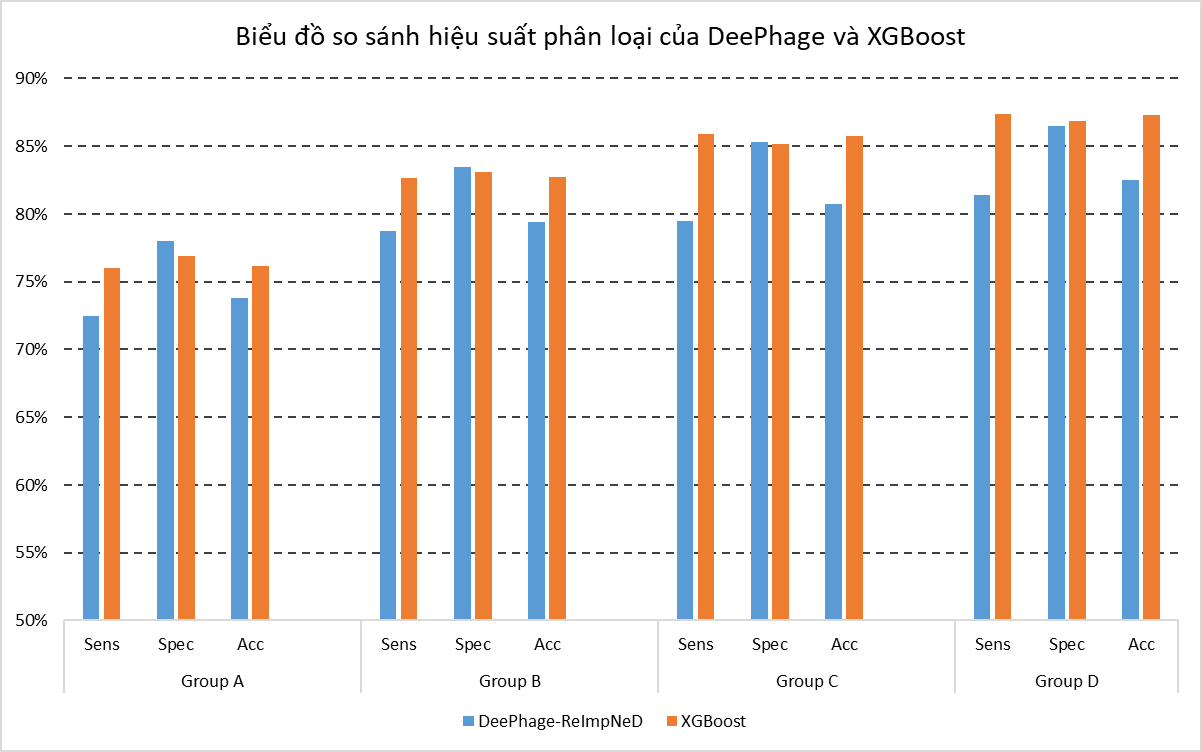
\includegraphics[width=1\linewidth]{figures/result_deephage_vs_xgboost.png}
    \caption{Kết quả hiệu suất phân loại của mô hình XGBoost trên tập dữ liệu xây dựng.}
    \label{fig:result_2}
\end{figure}

Hình \ref{fig:result_2} là biểu đồ so sánh hiệu suất phân loại của DeePhage và XGBoost trên tập dữ liệu mà nhóm sinh viên xây dựng. Có thể thấy, DeePhage cho kết quả tốt hơn 1 chút, khoảng từ 2\% - 5\% khi hơn XGBoost ở 2 chỉ số Sensitivity và Accuracy. Nghĩa là DeePhage cho khả năng nhận diện nhãn 1 và độ chính xác tổng thể cao hơn. Với chỉ số Specificity, XGBoost cho kết quả tốt hơn khoảng 5\%, nghĩa là khả năng nhận diễn nhãn 0 của XGBoost tốt hơn DeePhage.

